\section{Tense}

Grammatical tense is a category that expresses time reference with reference to the moment of speaking. In many languages there are three main categories of present, past and future, that refer to the moment of speaking, the period before and the period after it respectively. English is of the same group of languages with tense-rich grammar. It has 16 tenses, divided by categories of time and perfection. Novoslovnica has 12 tenses, based on the two principles like English. They are:

\begin{itemize}
	\item Present Indefinite Tense
	\item Present Definite Tense
	\item Future Indefinite Tense
	\item Future Definite Tense
	\item Pre-future Tense
	\item Future-in-the-Past Tense
	\item Pre-future-in-the-Past Tense
	\item Aorist
	\item Perfect
	\item Imperfect
	\item Plusquamperfect
	\item Past Indefinite Tense
\end{itemize}

First two tenses describe the present moment, the next three ones refers to the future period of time and the last six ones describe the period of time that has already passed.

We can divide past tenses in two groups - past tenses itself and future-in-the-past tenses, that describe actions that refer to the future moment with reference to the moment in the past.
Novoslovnica tense system can be described better with the help of the following diagram:

\begin{figure}
	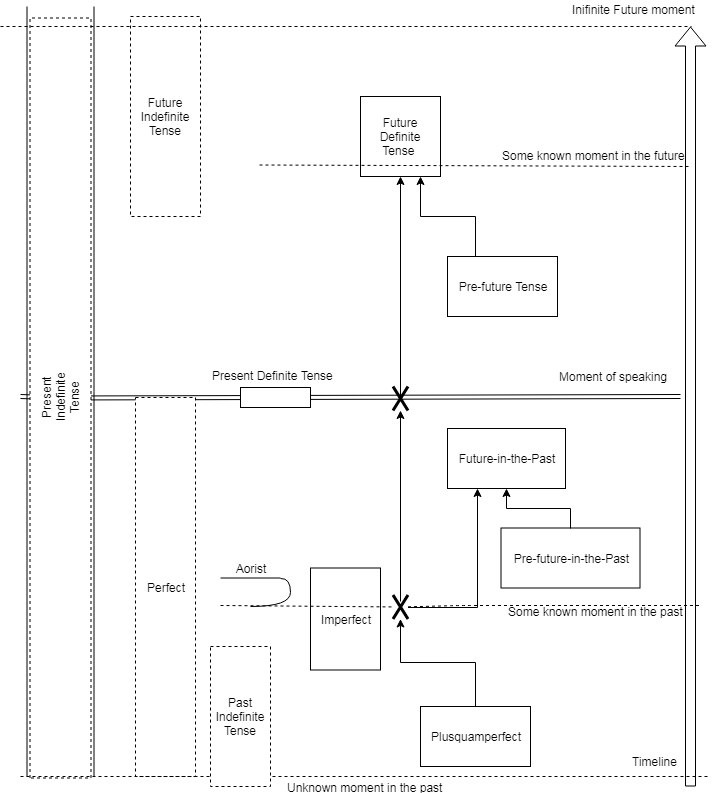
\includegraphics[width=\linewidth]{./sources/tenses.jpg}
	\caption{Tenses in Novoslovnica}
	\label{fig:tenses}
\end{figure}

Present group of tenses consists of Present Indefinite Tense (\textit{Pritomen čas}) and Present Definite Tense (\textit{Sëdyšen čas}).

Present Indefinite Tense (\textit{Pritomen čas}) is used when the action does not depend on time. For example, in the first example we know that the Earth always revolves and nothing but the apocalypsis can change it. This tense is very similar to the English one and has similar use cases. We can find this tense in indicative (examples 1, 2) and declarative (example 3, 4) moods mostly (in some cases it can be found in different moods too).

Note that in declarative there are two variants of present indefinite, because of its resultive semantics. In example 3 you can see the verb in declarative mood, in present indefinite tense, and in example 4 you can see the same tense and mood but within a predicateless sentence.

Also take care of the translation in example 3. You can mess it with English Present Perfect Tense (He has bought two cars), but this sentence should be translated with the verb «to have» in Present Indefinite with the participle III of the verb «to buy» (bought).

\textbf{Examples:}

\textit{Zemlä sę vreta okolo slånca.} - The Earth revolves around the Sun.

\textit{Vsękyǐ denj ja hođam do učilišta prez lěpyǐ park.} — Every day I walk to school through the beautiful park.

\textit{On imá kupeno dva vozidla.} — He has two cars bought.

\textit{Lěs i tïhota...} — There are forest and silence around me...

Present Definite Tense (\textit{Sëdyšen čas}) is used if the action depends on time. In the first example we can see a sentense with the following semantics: now I think about the rest, though in an hour I can forget about this thought.

Generally, this tense is close to Present Continuous Tense in English, though has a different interpretation. If you want to get in differences, we can give you such an example: «The sun is revolving around the Sun at the moment». Read this hypothetic sentence that is syntaxicly valid in English.

What would be the differences of English and Novoslovnica here? It is in a term of differentiation. English operates with the time and Novoslovnica operates with the mutability. That is why here Novoslovnica will still use Present Definite Tense with the word «sëdy» (at the moment).

\textbf{Examples:}

\textit{Ja myslü o počïvkě.} — I am thinking about the rest.

\textit{On idaje do råboty, zato ne može da odgovori vam.} — He is going to the work, that is why he cannot answer you.

The group of future tenses comprises two ones: Future Tense and Pre-future Tense.

Future Definite Tense (\textit{Bųdešt čas}) defines that the action will appear in the future with reference with the moment of speaking. There are three variants of how you can use Future Tense in Novoslovnica.

Firstly, you can use the verb «hteti» (to will) in 3-person form with the main verb in Present Indefinite Tense (example 1). This varitant is most similar to English Future Simple Tense.

Secondly, you can use the verb «byti» (to be) with inifinitive form of the main verb (example 2). This variant is close to English Future Continuous Tense. It is often used with verbs of A-type (read the chapter about verbal types in Novoslovnica).

Finally, you can use a synthetic verb form with the future tense conjugation (example 3). In English, it should be translated in Future Simple so as the first one.

\textbf{Examples:}

\textit{Ja hte kazam ti něčto.} — I will tell you something.

\textit{Ja bųdu sluhati gudbu.} — I will listen to music. (I will be listening to music).

\textit{Nakonec ja tę viđahtem}. – Finally, I will meet you.

Pre-future Tense (\textit{Predbųdešt čas}) is a grammatical tense that is used when the speaker should explicitly show that the action will take place before another future action. So, this tense deals with the comparison of future actions rather than with the moment of speaking.

In Novoslovnica Pre-future Tense is formed by using the verb «hteti» in 3-person form with the main verb in perfect form (examples 1, 2). This tense should be translated in English with Future Perfect Tense.

\textbf{Examples:}

\textit{Ja hte sòm kupil květy, dy ty hte priǐdaš do města.} — I will have bought flowers, when you will come to the place.

\textit{On hte je zakončil učilišto, dy otec mu hte sę vreta dodomu}. — He will have graduated from school, when his father will come back home.

Future Indefinite Tense (\textit{Něĝdašen čas}) is a rather rare tense to be used in Novoslovnica. It has no direct equivalents in English and should be translated in Future Simple with some keywords (such as «somewhen», «ever», «once»). The sense of this tense is to show that the action takes place in a future moment or period of time, but we do not care of when it will occur or how long it will last.
This tense is formed by Pre-future form of the verb «byti» with the past passive participle of the main verb. Look at the examples to get acquainted.

\textbf{Examples:}

\textit{On hte je byl nagrådil medalom mę.} — Once he will grant me with a medal.

\textit{Ja hte sòm byl kupil vašu věčj.} — Once I will but your item.

All other tenses are related to the past period of time. Firstly, we will consider real past tenses and then future-in-the-past ones.

Aorist (\textit{Prost minul čas}) determines the fact of the committed action without semantic details. It is similar in usage with English Past Simple Tense. Using Aorist we consider only the time the action occurs, but do not think about its duration.

In Novoslovnica it is formed by verb-base vowels with past definite endings: «-h», «-ša», «-še», «-hma», «-hta», «-ha», «-hme», «-hte», «-hu».

\textbf{Examples:}

\textit{Ja dělah råbotu-ta včera.} — I did the work yesterday.

\textit{Pred dvě ročiny ja jěŝih v gråd-òt.} — Two years ago I travelled to the city.

Imperfect (\textit{Neporęden minul čas}) determines the imperfect aspect of the past action. That means it is used with habitual, durable repeated actions etc, that took place in the past. Using imperfect we add the information, that our action took some exact time in the past. This tense is similar in usage with English Past Continuous Tense or Past Perfect.

It is formed so as Aorist with the one difference. There is a «-ě-» vowel before endings, not the verb-base vowel. So, for any verb type (see a chapter about verbal types) there is only a single imperfect form.

\textbf{Examples:}

\textit{Ja pišěh nadomnu råbotu dvě godiny včera.} — I was writing my homework for two hours yesterday.

\textit{Prijatelj mi ráděše na zavodu dvě ročiny.} — My friend had worked on a plant for two years.

Perfect (\textit{Svòršen minul čas}) determines the action has been committed before the present moment. That means, that we take account on the result of the action, on the fact it is finished, while Aorist determines the fact of the action itself and the time when it occured. So, it is a full equivalent of English Present Perfect Tense.

In Novoslovnica Perfect is formed by the auxiliary verb «byti» in Present Indefinite and an L-participle following it.

\textbf{Examples:}

\textit{On je izmyslïl novu ŧeoriju o problemě-ta.} — He has devised a new theory on the problem.

\textit{Môǐ brat je zakončil vysšojučilišto.} — My brother has graduated from University.

Plusquamperfect (\textit{Predminul čas}) determines the fact our action is further from us than another action in the past. It is akin Pre-Future tense, just with past actions. Simply speaking, it is an equivalent of English Past Perfect Tense. So as Pre-Future tense, actions in Plusquamperfect are usually used in pair with another past action that stands in Aorist.

Plusquamperfect in Novoslovnica is formed with aorist form of the auxiliary verb «byti» with an L-participle of the main verb.

\textbf{Examples:}

\textit{Ja byh doǐdal do ulicy-ta, dy on mi odŝvoniše, če ne može da priǐde.} — I had arrived to the street by the time he called be to say he cannot come.

\textit{On byše zdělal model, ĝda ja kazaše mu, če to ne máše potrěbnostï.}

Now we should consider two last tenses: Future-in-the-Past tense and Pre-Future-in-the-Past tense.
Future-in-the-Past tense (Bųdešt v minulom čas) is used when we speak about past actions, that occured after some other past actions. To emphasize this fact we use a past variant of the future tense — Future-in-the-Past. English has an equivalent, so it is easy to build a parallel between these two ones. In Novoslovnica this time is build with imperfect of the auxiliary verb «hteti» and DA-construction of the main verb (example 1).

This tense has also another meaning, that can be expressed with «would like to» phrase in English. It shows a polite intention to do something (example 2).

\textbf{Examples:}

\textit{My zapytahme dali vozidlo htěše da priǐde včas.} — We wondered if the bus would arrive on time.

\textit{Ja htěh da kazam ti něčto.} — I would like to say you something.

Pre-Future-in-the-Past tense (\textit{Predbųdešt v minulom čas}) is used, when we speak about some actions, that happened earlier than some future actions in the past (analogue of pre-future tense in the past). It has a similar meaning with Future-in-the-Past Perfect tense in English and it is rather rarely used.

It is formed with imperfect of the auxiliary verb «hteti» with perfect form of the main verb via DA-construction (look at the example).

\textbf{Examples:}

\textit{Vy kazahte, če htěhte da jeste podpisali pismo pred tym, kak htěhte da započïnate råbotati.} — You said you would have signed the paper before you would start working.

Past Indefinite Tense (\textit{Davnominul čas}) is the last official tense in Novoslovnica. It describes an action that occured in some moment in the past we do not know. In English we should translate it with Past Simple or with the «used to»-construction. It can be considered as a pair to Future Indefinite Tense.

\textbf{Examples:}

\textit{On je byl pisal knigu.} — He used to write a book.

Let us summarize all the equivalents of Novoslovnica's Tenses in English in the next table.

\begin{table}
	\caption{English equivalents of tenses in Novoslovnica}
	\begin{tabular}{ p{11em} p{11em} }
		\textbf{Tense in Novoslovnica}       & \textbf{English equivalent}                  \\
		Present Indefinite Tense             & Present Simple                               \\
		Present Definite Tense               & Present Continuous                           \\
		Future Indefinite Tense              & “once” + Future Simple                       \\
		Future Definite Tense (with “hteti”) & Future Simple                                \\
		Future Definite Tense (with “byti”)  & Future Continuous                            \\
		Future Definite Tense (single form)  & Future Simple                                \\
		Pre-future Tense                     & Future Perfect (Cont.)                       \\
		Future-in-the-Past Tense             & Future-in-the-Past Simple or “would like to” \\
		Pre-future-in-the-Past Tense         & Future-in-the-Past Perfect (Cont.)           \\
		Aorist                               & Past Simple                                  \\
		Perfect                              & Present Perfect (Cont.)                      \\
		Imperfect                            & Past Continuous                              \\
		Plusquamperfect                      & Past Perfect (Cont.)                         \\
		Past Indefinite Tense                & “used to”                                    
	\end{tabular}
\end{table}

The third verbal category can be found in Novoslovnica which is shown only in differences between Aorist and Imperfect: perfection, while other tenses differ only by determinacy and time. So, you can use complex tenses as Perfect, Plusquamperfect, Past Indefinite etc. with aorist and imperfect participles and receive two shades of perfection meaning.
